\section{Beschreibung des User Interface Konzepts}

\subsection{Desktop Web Interface}

\subsubsection{Navigation} \label{subsubsection:navigation}

\begin{figure}[htl]
\centering
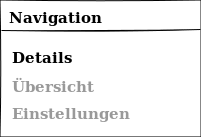
\includegraphics[width=4cm]{img/web_navigation}
\caption{Navigationsleiste}
\label{fig:web_navigation}
\end{figure}

Die Navigationsleiste wird auf jedem Screen entlang der linken Bildschirmkante
angezeigt. Sie stellt eine Navigationshierarchie dar, die vom Benutzer geklickt
werden kann. Das aktuelle Element wird nach Applikationskonvention schwarz
dargestellt, andere Seiten dunkelgrau.  Momentan ist die Navigation relativ
spärlich besetzt, sie bietet aber reichlich Platz für eventuelle Erweiterungen
der Applikation.

\subsubsection{Aktuelles Monat} \label{subsubsection:aktuelles_monat}

\begin{figure}[htl]
\centering
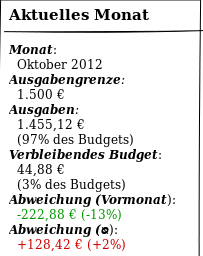
\includegraphics[width=4cm]{img/web_current_month}
\caption{Aktuelles Monat}
\label{fig:web_current_month}
\end{figure}

\"Ahnlich zur Navigationsleiste wird auf jedem Screen unten entlang der linken
Bildschirmkante eine kurze Zusammenfassung des aktuellen Monats dargestellt.
Der Benutzer erfährt auf einen Blick wichtige Kennzahlen wie zum Beispiel die
aktuell eingestellt Budgetgrenze, die bisherigen Monatsausgaben, das
verbleibende Budget, und Vergleiche mit dem Vormonat beziehungsweise dem
Durchschnitt aller Monate.

Wenn möglich werden diese Kennzahlen sowohl als Absolutbetrag sowie als
Prozentzahl dargestellt. Negative Abweichungen werden grün dargestellt (= man
hat im Vergleich dieses Monat gespart), positive mit roter Schriftfarbe.

Wenn Horst sich einloggt, kann er über die Monats\"ubersicht sofort sehen,
wieviel er bereits ausgegeben hat und wie viel Geld ihm in diesem Monat noch
bleibt.

\subsubsection{Details}

\begin{figure}[htl]
\centering
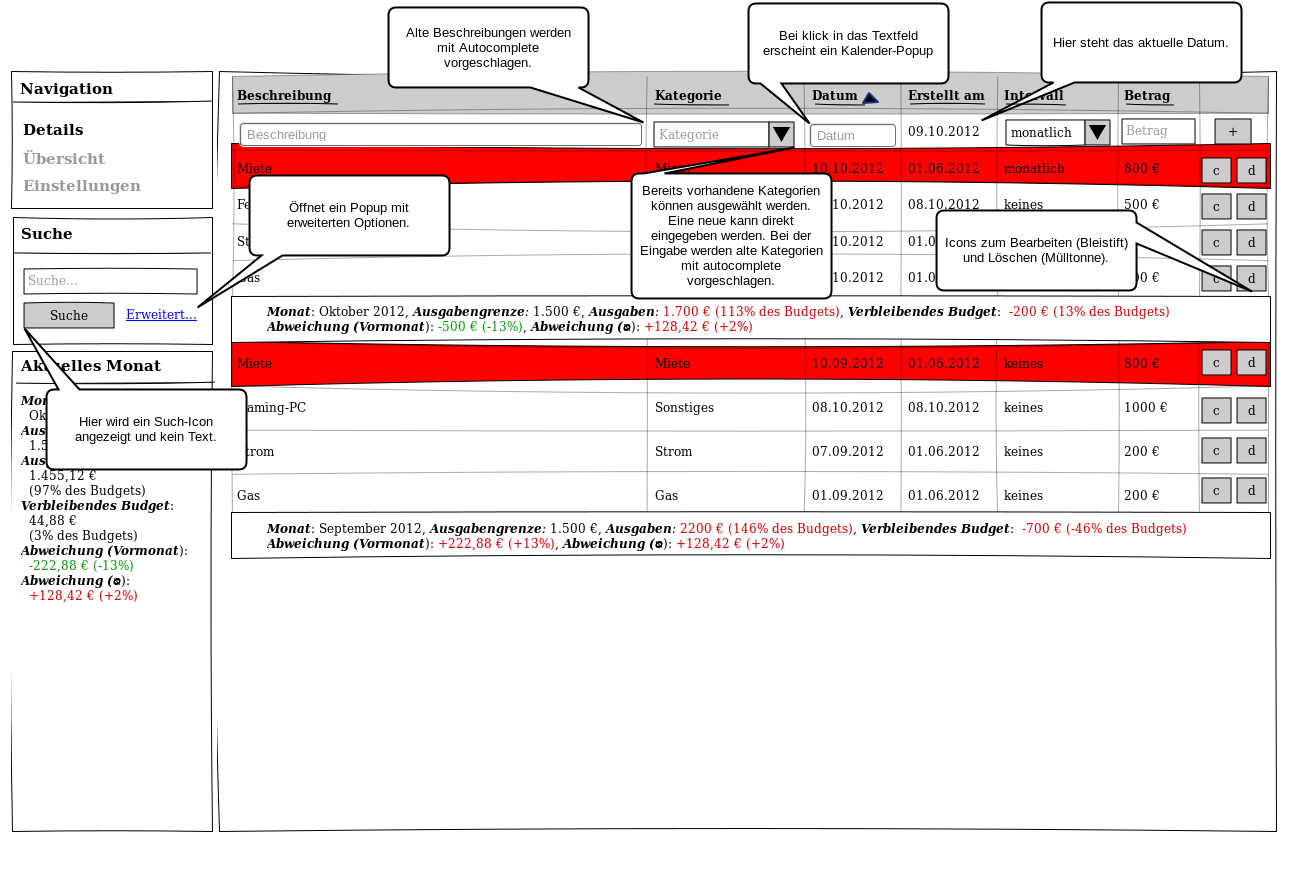
\includegraphics[width=\textwidth]{img/web_details}
\caption{Web Details}
\label{fig:web_details}
\end{figure}

Die Detailansicht enthält eine komplette Auflistung aller eingetragenen Ausgaben, dargestellt
in einem Tabellenformat. Als Spalten werden angezeigt:

\begin{itemize}
    \item die Beschreibung des Eintrags,
    \item die Kategorie,
    \item das Datum,
    \item das Erstellungsdatum,
    \item das Intervall (bei wiederkehrenden Ausgaben),
    \item und der Betrag.
\end{itemize}

Per Default ist die Liste nach absteigend nach Datum sortiert. In dieser Sortierung wird nach den
Einträgen jeden Monats eine Zusammenfassungszeile angezeigt mit relevanten Informationen wie der Summe von Ausgaben dieses Monats u.ä.

Auch bei anderen Sortierungen kann teilweise eine Zusammenfassungszeile angezeigt werden; zum Beispiel ist auch
bei Sortierung nach Kategorie die Summe aller Ausgaben von Interesse.

Jeder Eintrag kann auch durch einen Click auf die Buttons am rechten Zeilenende editiert oder gelöscht werden.
Zum Editieren wird ein inline Editor verwendet damit der Benutzer sich nicht neu orientieren muss.

Wiederkehrende Ausgaben werden ebenfalls in dieser Liste dargestellt. Sobald eine wiederkehrende Ausgabe getätigt wurde
(also das aktuelle Datum nach dem nächsten Eintreffen dieser Ausgabe ist), wird ein neuer Eintrag \emph{ohne} einem Intervall
erzeugt. Es besteht also zu jeder wiederkehrenden Ausgabe immer jeweils nur ein 'wiederkehrender' Eintrag, aber beliebig viele
nicht-wiederkehrende Einträge.

Neue Einträge werden am oberen Ende der Liste mit einem inline Editor erstellt. Es wird Auto-Complete verwendet um fehlerhafte
Eingaben zu reduzieren. Sobald der Focus auf Datumseinträge fällt wird ein Kalenderwidget als Popup angezeigt (ähnlich wie bei der
OEBB Streckensuche). Ebenfalls können Intervalle durch eine Drop-Down-Liste spezifiziert werden. Bei Formatierungsfehlern wird ein 'Fehler' Icon mit entsprechendem Mouse-Over Text angezeigt. Durch einen Click
auf den 'Add' Button auf der rechten Seite der Zeile wird der Eintrag
schließlich erstellt.

M\"ochte Horst nun die Rechnung seines Pakets eintragen, trägt er einfach die
verschiedenen Positionen in der 1. Zeile der Detailansicht ein und klickt danach
auf die \glqq +\grqq-Taste. Gleichzeitig kann Horst sofort erkennen, wenn er das
festgelegte Budget \"ubertritt, da jeder Eintrag, der das Budget übersteigt
rot angezeigt wird.

\begin{figure}[htl]
\centering
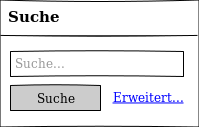
\includegraphics[width=4cm]{img/web_simple_search}
\caption{Einfache Suche (Ausschnitt aus der Detail Ansicht)}
\label{fig:web_simple_search}
\end{figure}

\begin{figure}[htl]
\centering
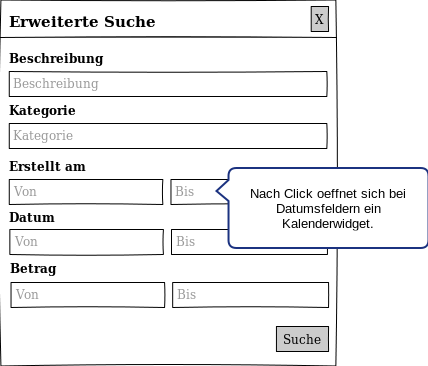
\includegraphics[width=4cm]{img/web_advanced_search}
\caption{Erweiterte Suche (Popup nach Click auf 'Erweitert...' in der Einfachen Suche)}
\label{fig:web_advanced_search}
\end{figure}

\begin{figure}[htl]
\centering
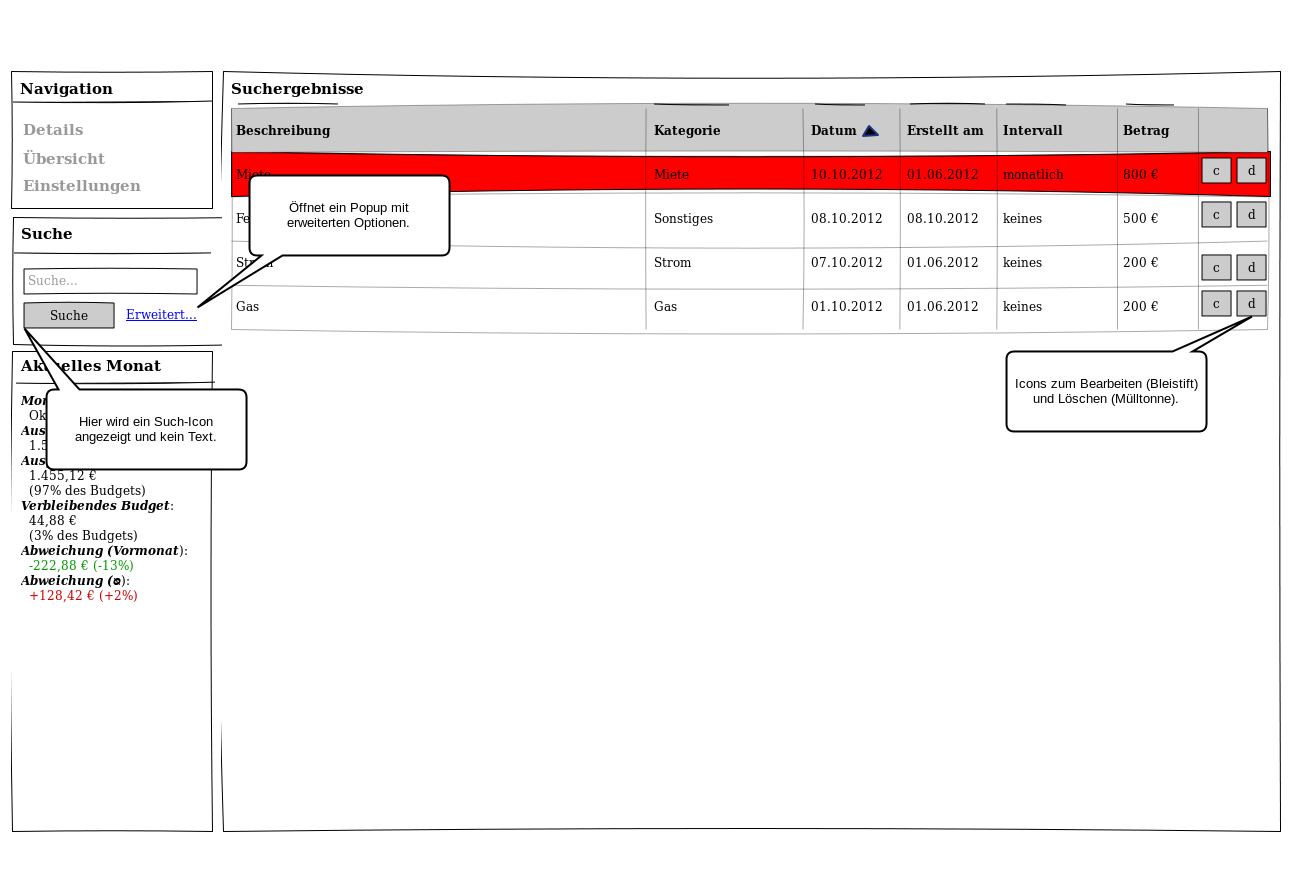
\includegraphics[width=\textwidth]{img/web_search}
\caption{Suchergebnisse (Geladen nach Click auf den 'Suche' Button)}
\label{fig:web_search}
\end{figure}

Auf der linken Seite ist zusätzlich zur Navigation und der Monatszusammenfassung (siehe Abschnitt \ref{subsubsection:navigation} und \ref{subsubsection:aktuelles_monat}) ein Suchfeld. Es gibt einerseits die einfache Suche (Abbildung \ref{fig:web_simple_search}, eine Textsuche durch Kategorie und Monat), und andererseits nach einem Click auf
'Erweitert...' eine erweiterte Suche (Abbildung \ref{fig:web_advanced_search}). Diese bietet außer der simplen Textsuche eine Bereichssuche für den Betrag (zum Beispiel 'zwischen 300 und 500 Euro') und das Datum. Suchergebnisse werden in einem separaten Screen (Abbildung \ref{fig:web_search}) im selben Format wie die Details angezeigt.

\subsubsection{Übersicht}

\begin{figure}[htl]
\centering
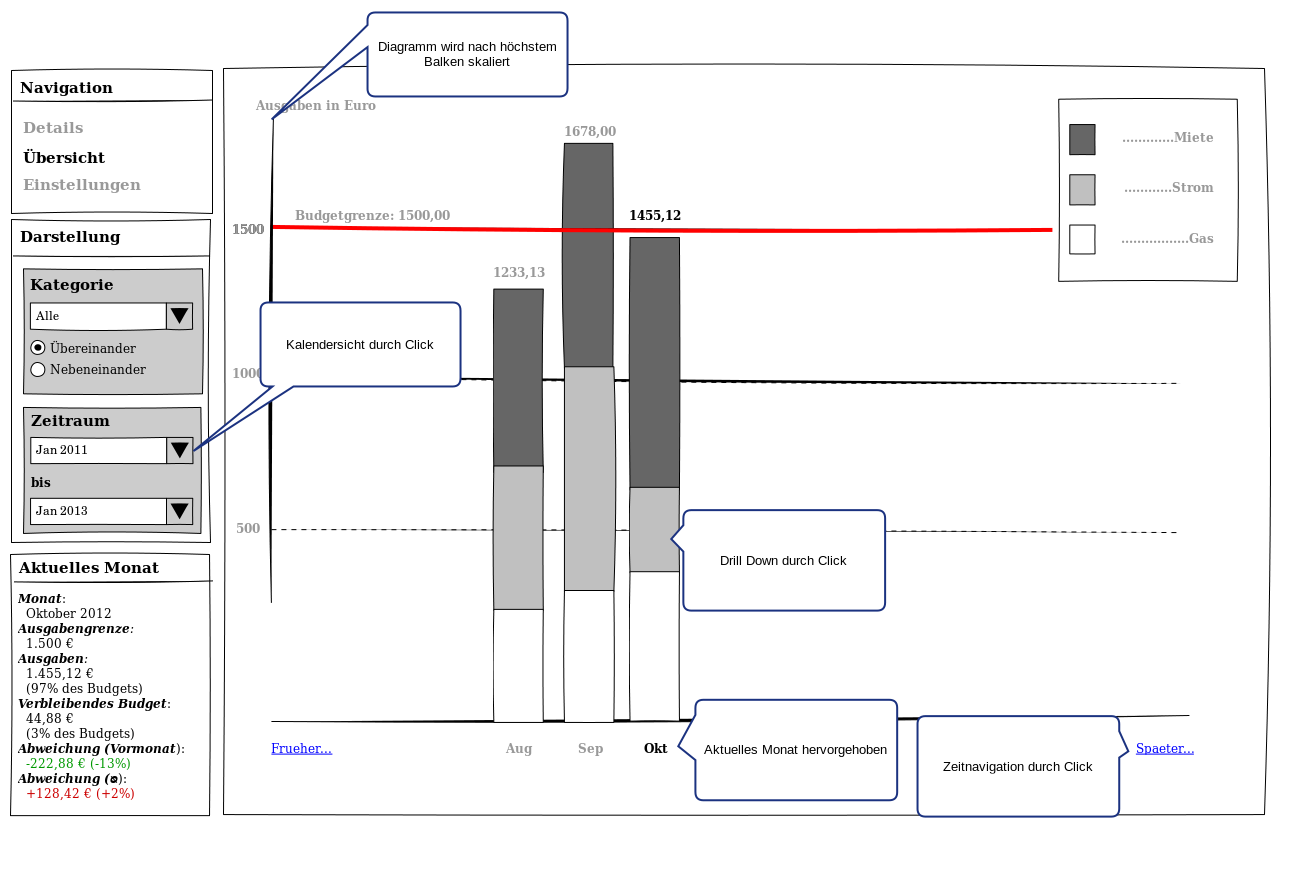
\includegraphics[width=\textwidth]{img/web_uebersicht}
\caption{Web \"Ubersicht}
\label{fig:web_uebersicht}
\end{figure}

In der Übersicht (Abbildung \ref{fig:web_uebersicht}) werden aggregierte Informationen zu den Finanzen dargestellt.
Dieser Screen kann durch einen Click auf 'Übersicht' innerhalb der
Navigationsleiste erreicht werden.

Auf der linken Seite des Bildschirms wird weiterhin (nach
Applikationskonvention) oben die Navigationsleiste (siehe Abschnitt
\ref{subsubsection:navigation}), und unten eine Zusammenfassung des aktuellen
Monats (siehe Abschnitt \ref{subsubsection:aktuelles_monat}) angezeigt.
Zusätzlich dazu werden nun Konfigurationsmöglichkeiten der
Übersichtsdarstel\-lung angeboten, mithilfe dessen die Diagramme an
Benutzerpräferenzen angepasst werden können (Abbildung \ref{fig:web_display_settings}).

\begin{figure}[htl]
\centering
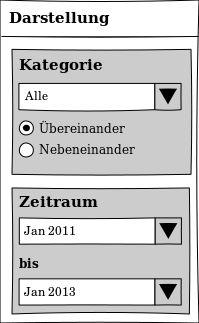
\includegraphics[width=4cm]{img/web_display_settings}
\caption{Darstellungseinstellungen}
\label{fig:web_display_settings}
\end{figure}

Es können die angezeigten Kategorien gefiltert werden; entweder werden alle
Kategorien angezeigt, oder man beschränkt sich auf eine bestimmte Kategorie.
Die Kategorieauswahl kann ebenfalls durch einen Click auf einen Balken
innerhalb des Diagramms getätigt werden. Die Darstellung der Kategorien kann
durch Radiobuttons entweder übereinander oder nebeneinander\footnote{Besonders
nützlich für Vergleiche zwischen Kategorien.} konfiguriert werden.  Wenn eine
bestimmte Kategorie ausgewählt ist werden die Radiobuttons ausgeblendet.

Es besteht außerdem die Möglichkeit zur Einstellung des angezeigten Zeitraums.
Durch einen Click auf eine der Zeitauswahlkomboboxen öffnet sich eine
Kalenderansicht. Der Zeitraum kann ebenfalls durch die Links 'Früher' und
'Später' im Diagramm geändert werden. Dadurch vergrößert sich der Zeitrahmen um
3 Monate in die jeweilige Richtung.

Das Diagramm selbst stellt Ausgaben (aggregiert nach Kategorie) pro Monat dar.
Die Diagrammskala wird jeweils nach dem höchsten Balken skaliert.  Die
eingestellte Budgetgrenze wird durch eine rote Linie dargestellt (falls sie
innerhalb das skalierte Diagramm fällt). Kategorien werden durch Farbkodierung
unterschieden, welche in der Legende aufgeschlüsselt ist. Achsen sind
selbstverständlich beschriftet; in der Monatsbeschriftung wird das aktuelle
Monat farblich hervorgehoben\footnote{Nach Applikationskonvention ist das
aktuelle Element schwarz, und alle anderen dunkelgrau}.

Wenn Horst sehen m\"ochte wieviel er f\"ur jede Kategorie im Vergleich
ausgegeben hat, kann er einfach \glqq nebeneinander\grqq\space ausw\"ahlen und sieht
dann die Balken der Kategorien f\"ur jedes Monat nebeneinander. So kann er
sofort erkennen, dass er f\"ur seine Wohnung in diesem Monat den gr\"o\ss ten
Teil seines Budgets ausgegeben hat.

\newpage
\subsubsection{Einstellungen}

\begin{figure}[htl]
\centering
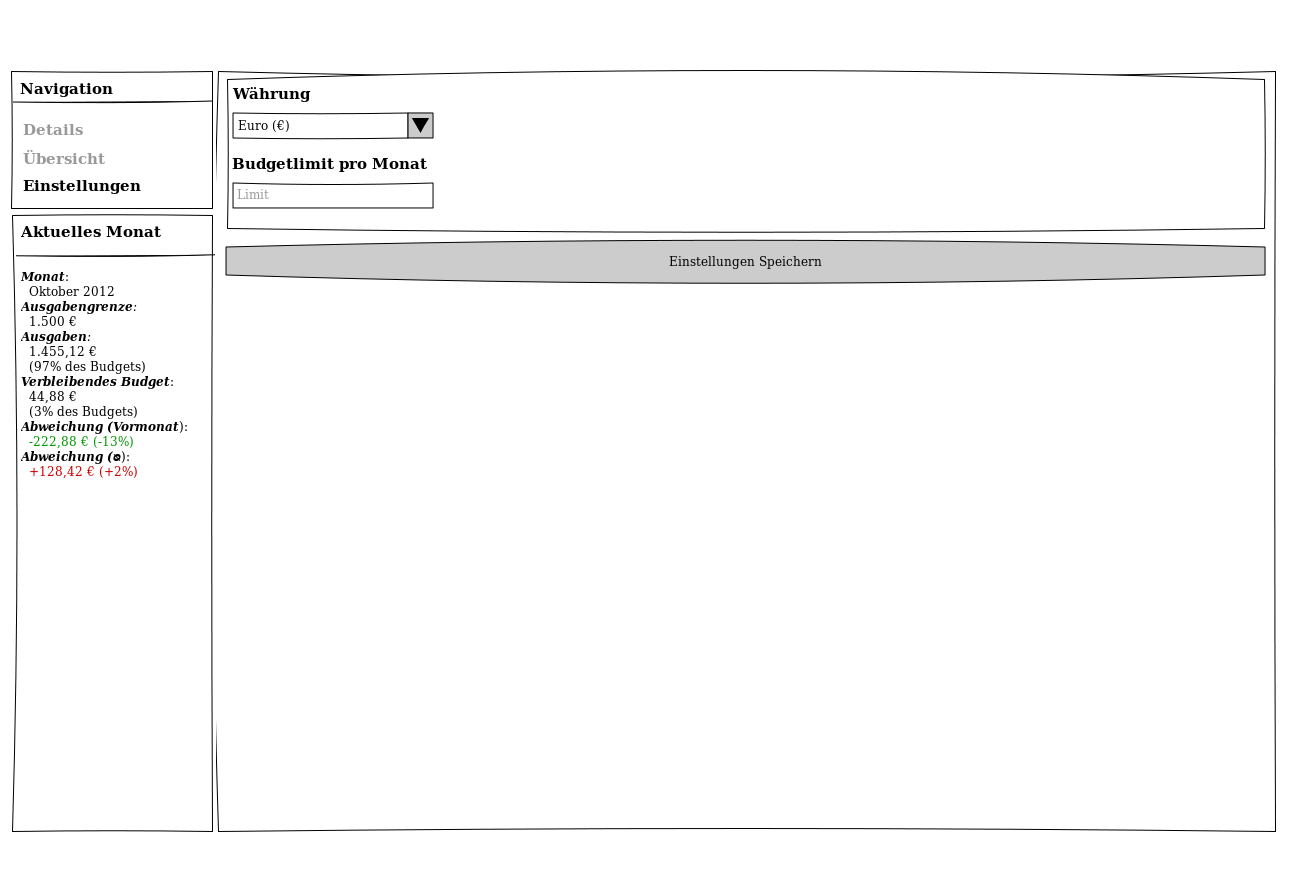
\includegraphics[width=\textwidth]{img/web_settings}
\caption{Web Einstellungen}
\label{fig:web_settings}
\end{figure}

Unter Einstellungen kann man die W\"ahrung und das Budget setzen. Falsche
Einstellungen werden dadurch vermieden, dass die W\"ahrung nur aus einer
Combo-Box ausgew\"ahlt werden k\"onnen.

Wenn Horst eine Gehaltserh\"ohung bekommt, kann er hier das Budget entsprechend
anpassen.

\subsubsection{Resume}

Die aktuelle Form der L\"osung wurde aus Gründen der Einfachheit (= Simplicity) und leichten Verst\"andlichkeit gew\"ahlt.
Es gibt nur zwei Hauptbereiche der Applikation, deren Verwendung klar ersichtlich ist.
Alle erwarteten Workflows sollten sich mit wenig Aufwand durchf\"uhren lassen.

Innerhalb dieser Applikation wird besonders Wert auf Konsistenz gelegt um nicht gegen die Erwartungen
von m\"oglicherweise unerfahrenen Benutzern wie Horst und Frauke zu versto\ss en. Beispiele daf\"ur sind
zum Beispiel die Verwendung von Hintergrundfarben (Rot bedeutet '\"uberzogen', Gr\"un 'nicht \"uberzogen)m
und das Hervorheben von Elementen durch die Verwendung von Schwarz und Dunkelgrau.

Es wird auch versucht Aktionen so einfach wie m\"oglich zu halten. Buttons verwenden f\"ur Funktionen wie
Suche, Neuer Eintrag, Eintrag \"Andern und Eintrag L\"oschen Standards-Icons die fast allen Benutzern gel\"aufig sind.
Dadurch sind einfache Handlungen selbsterkl\"arend und haben eine gute visuelle Affordance.

Das Poka-Yoke Prinzip kam beim Design der Applikation ebenfalls zur Anwendung. Soweit
wie m\"oglich werden Fehler in der Bedienung durch eingeschr\"ankte Eingabem\"oglichkeiten (wie zum Beispiel dem
Kalenderwidget) vermieden.

\subsection{Mobiles User Interface}

Beim Smartphone-GUI geht es vor allem darum, die im Vergleich eher spärlich
vorhandene Fläche effizient und intuitiv bedienbar zu gestalten. Da die vollstän\-dige Portierung aller Funktionen, die in der Web-Applikation zur Verfügung stehen, zu relativ vielen Einzelnen Screens geführt, und somit die Übersicht stark beeinträchtigt hätte, beschränkt sich die Smartphone-App auf wesentliche Funktionen. Allen voran sind das die Zusammenfassung der wichtigsten Kennzahlen, die gleich nach dem Login auf der Startseite aufscheint und die Eingabe, die für nicht wiederkehrende Ausgaben wohl hauptsächlich am Smartphone durchgeführt wird (Lebensmitteleinkäufe usw.). Weiters gibt es eine Liste mit den kürzlich erfassten Ausgaben, über die man durch Klick auf ein Listenelement dieses nachträglich noch bearbeiten kann. Weiters gibt es eine Ansicht mit einer einfachen Monatsstatistik in Form eines Säulendiagramms,
Verzichtet wurde hingegen auf eine Möglichkeit der Suche, einer genaueren Auswertung sowie auf die Erstellung wiederkehrender Ausgaben, da sie die Einfachheit („Simplicity“) unnötig beeinträchtigen würden und viel bequemer am Web-Interface bedient werden können. Die Smartphone-App ist also mehr als eine Ergänzung zum bereits sehr mächtigen Web-Interface zu sehen, mit der Horst und Frauke einerseits sehr schnell Vorort über potenzielle Ausgaben entscheiden können („Geht sich das Smartphone für meine Frau diesen Monat noch aus?“), andererseits nach getätigten Einkäufen diese sofort erfassen, und sich somit die Aufbewahrung der Rechnung ersparen können.

\subsubsection{Navigation}

Die Navigation erfolgt, Smartphone-typisch hierarchisch. Ausgehend von dem Startscreen mit der Kennzahlenzusammenfassung gelangt man in die Listenansicht und in die Neuerfassung. Nach erfolgter Neuerfassung gelangt man in die Listenansicht, durch den zur\"uck-Button wieder auf den Startscreen. Von der Listenansicht kommt man durch Klick auf ein Listenelement in dessen Bearbeitungsansicht, durch Klick auf den Statistik-Button in die Statistikansicht. Durch den Zur\"uckbutton jeweils wieder in die n\"achsth\"ohergelegene Ansicht.

\subsubsection{Login}

\begin{figure}[htl]
\centering
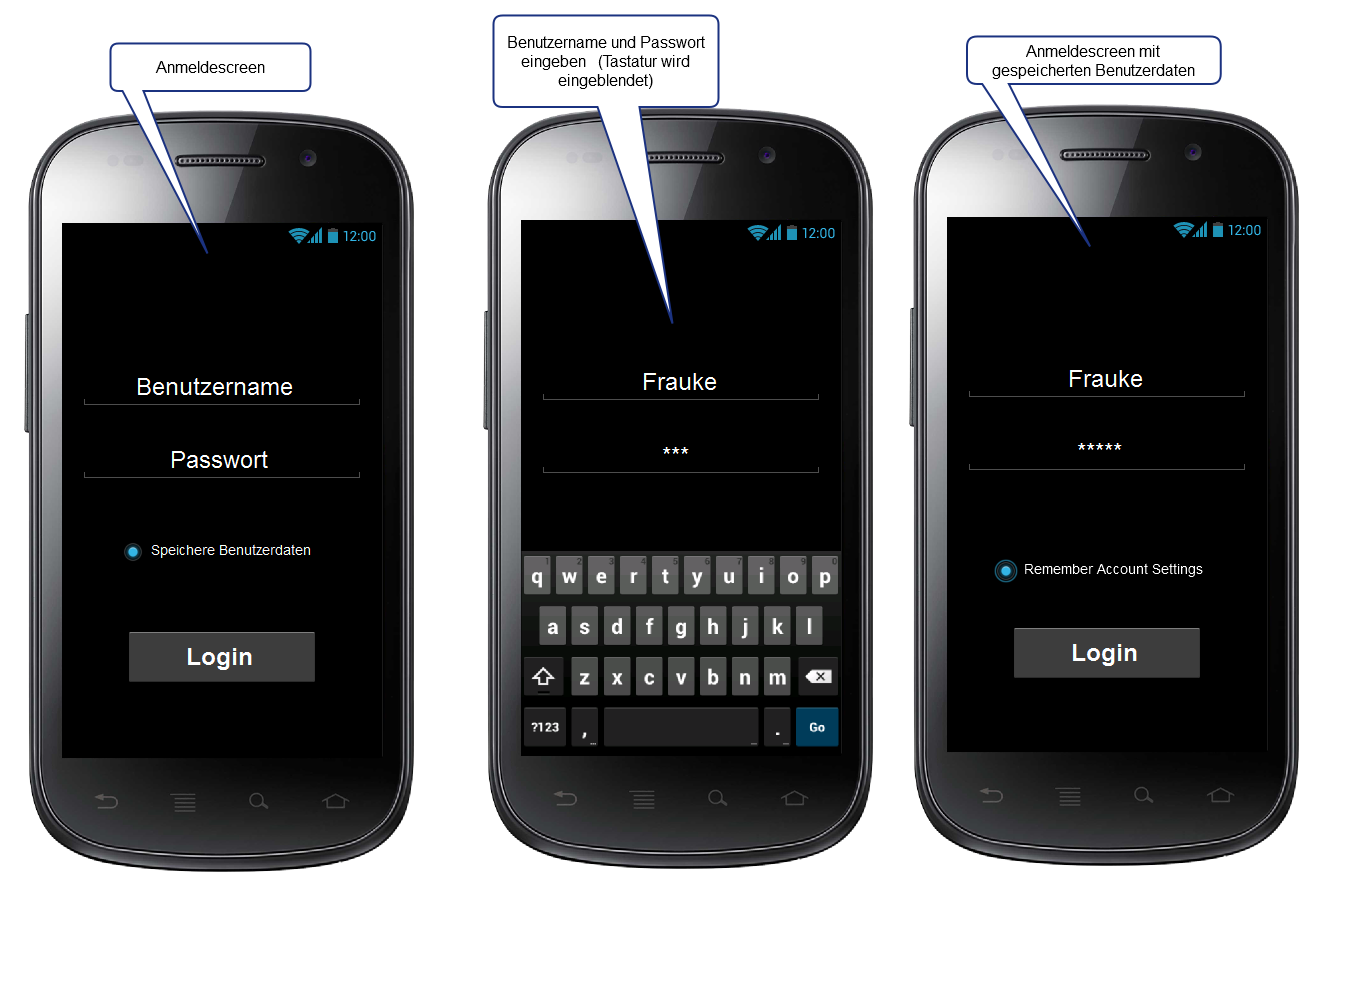
\includegraphics[width=\textwidth]{img/LoginScreen}
\caption{Login Screen}
\label{fig:login_screen}
\end{figure}

Ein Login ist erforderlich zur Synchronisierung mit der Web-Applikation, die Authentifizierung erfolgt nat\"urlich per Benutzername-Passwort Kombination, diese kann gespeichert werden, was dazu führt, dass das n\"achste mal der Loginscreen nicht mehr erscheint und direkt die Zusammenfassungsseite ge\"offnet wird.

\subsubsection{Startscreen}

\begin{figure}[htl]
\centering
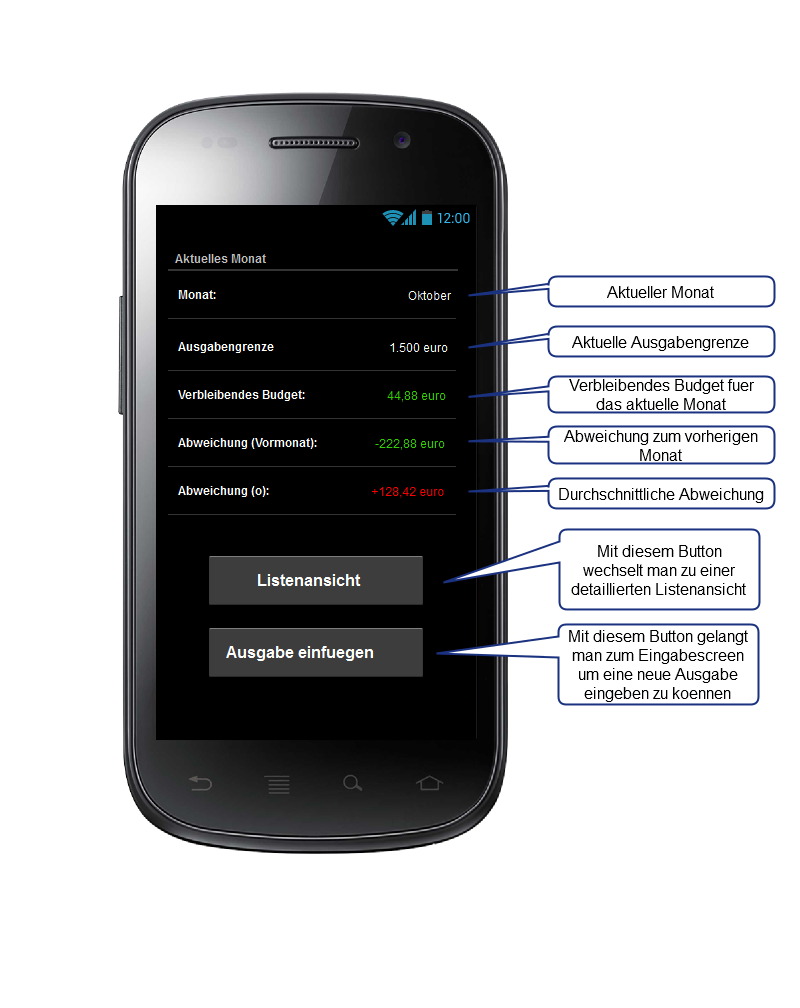
\includegraphics[width=5cm]{img/TitelScreen}
\caption{Start Screen}
\label{fig:start_screen}
\end{figure}

Wie gut zu erkennen ist, sind am Startscreen die wesentlichen Kennzahlen zusammengefasst, wie schon aus der Webapplikation bekannt. Dies ermöglicht einen sehr schnellen Überblick und erleichtert sehr stark die Entscheidung über einen möglichen Einkauf. Weiters gibt es 2 Navigationsbuttons, über die man in der Navigationshierarchie weiter hinunter navigieren kann.

\subsubsection{Eingabescreen}

\begin{figure}[htl]
\centering
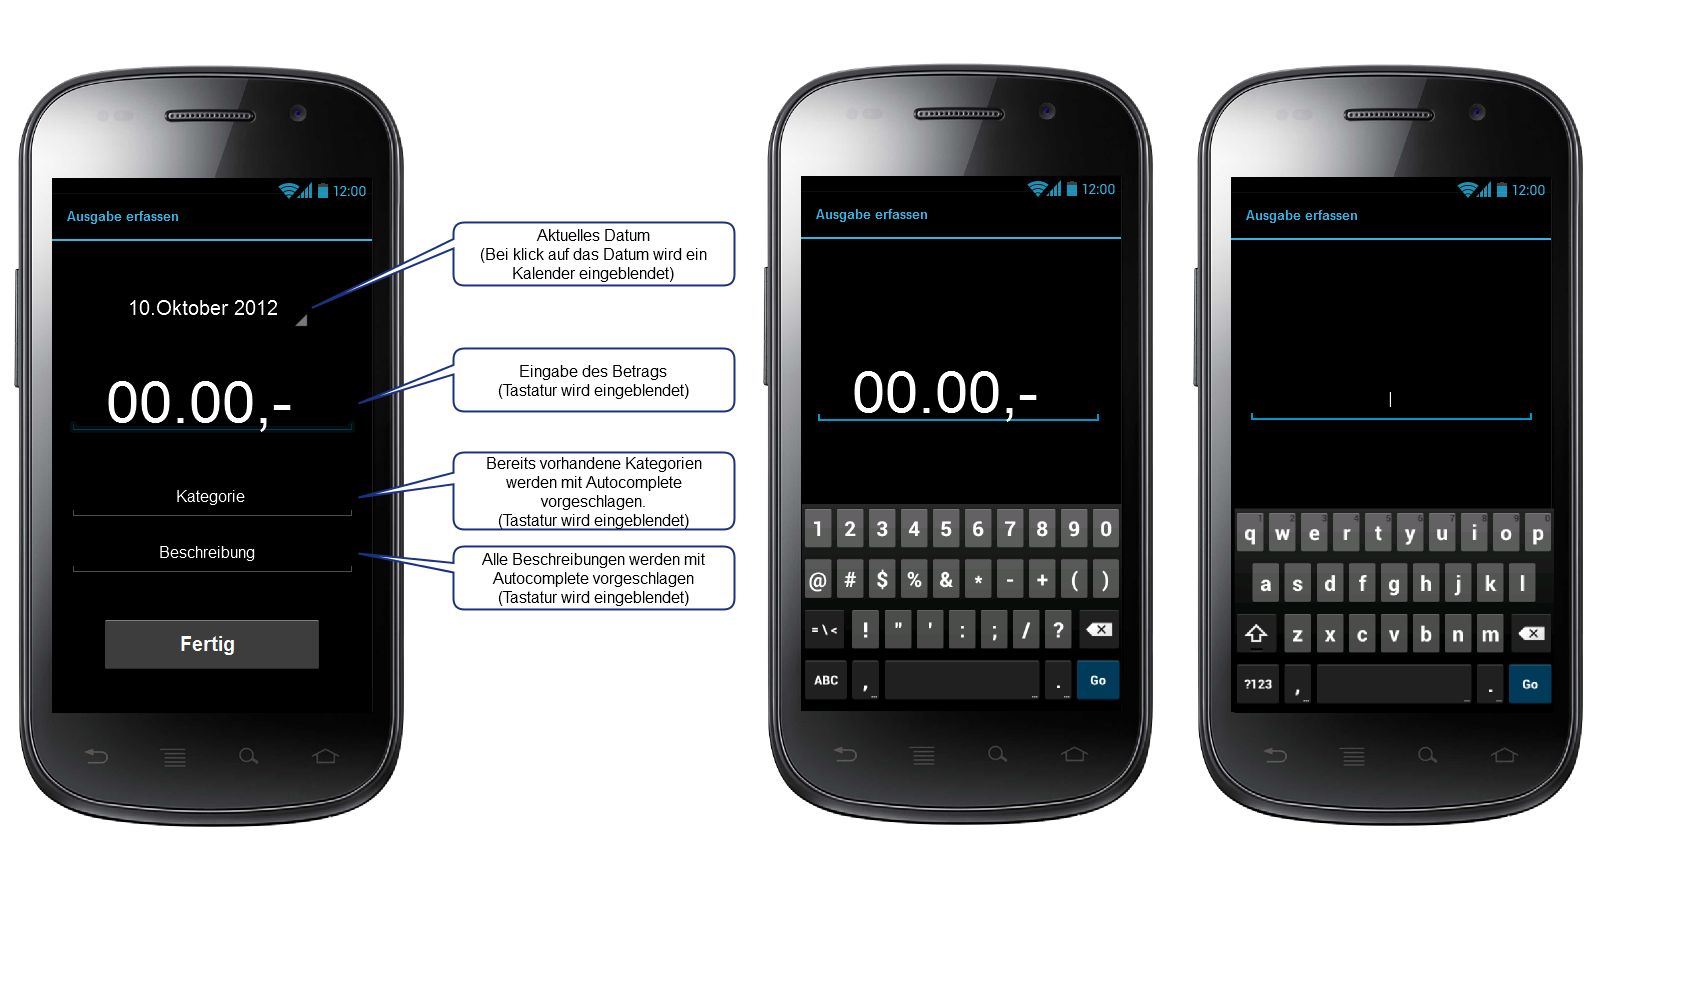
\includegraphics[width=\textwidth]{img/EingabeScreen}
\caption{Eingabe Screen}
\label{fig:eingabe_screen}
\end{figure}

Hier erfolgt die Ausgabenerfassung. Standardm\"aßig ist das aktuelle Datum eingestellt, was wohl in 95\% der Smartphone-Benutzungen so stehen bleibt, da man bereits vergangene oder zukünftige Ausgaben vorgesehenerweise eher über das Web-Interface eingibt. Der Preis, als wichtigstes Informationselement ist hervorgehoben. Kategorie und Beschreibung fragen, wie beim Web-Interface, während der Eingabe vorhandene Datens\"atze ab und erm\"oglichen durch Autovervollständigung eine effiziente Eingabe.

\subsubsection{Listenansicht}

\begin{figure}[htl]
\centering
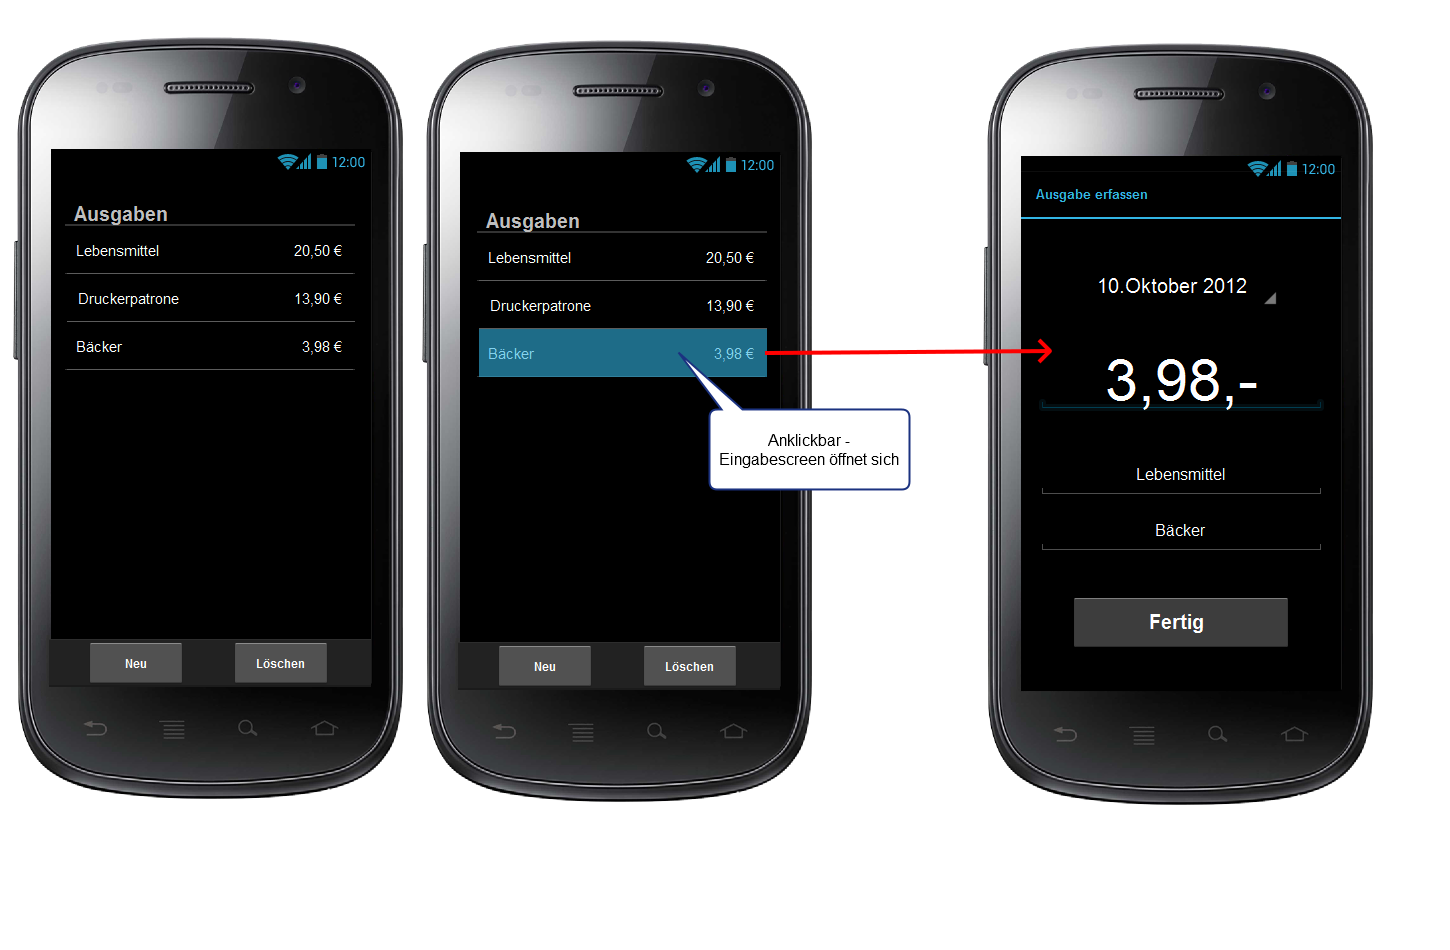
\includegraphics[width=\textwidth]{img/Liste}
\caption{Listenansicht}
\label{fig:listen_ansicht}
\end{figure}

Hier werden kürzlich getätigte Ausgaben aufgelistet, durch Klick kommt man in den Bearbeitungsmodus. Weiters gibt es 3 Buttons: Neu ermöglicht eine neue Eingabe, Löschen lässt neben allen Listenelementen einen X-Button erscheinen, durch dessen betätigung das jeweilige Element gelöscht wird. Statistik öffnet den Statistik-Screen. Die Smartphone-Liste ist wesentlich einfacher gehalten, als die Web-Liste. Die Schlüsseldaten „Beschreibung“ und „Preis“ reichen gew\"ohnlich in Verbindung mit der rückwärts-chronologischen Sortierung zur schnellen Identifizierung kürzlich getätigter Ausgaben. So bleibt die Liste übersichtlich und smartphonegerecht.

\subsubsection{Statistikansicht}

\begin{figure}[htl]
\centering
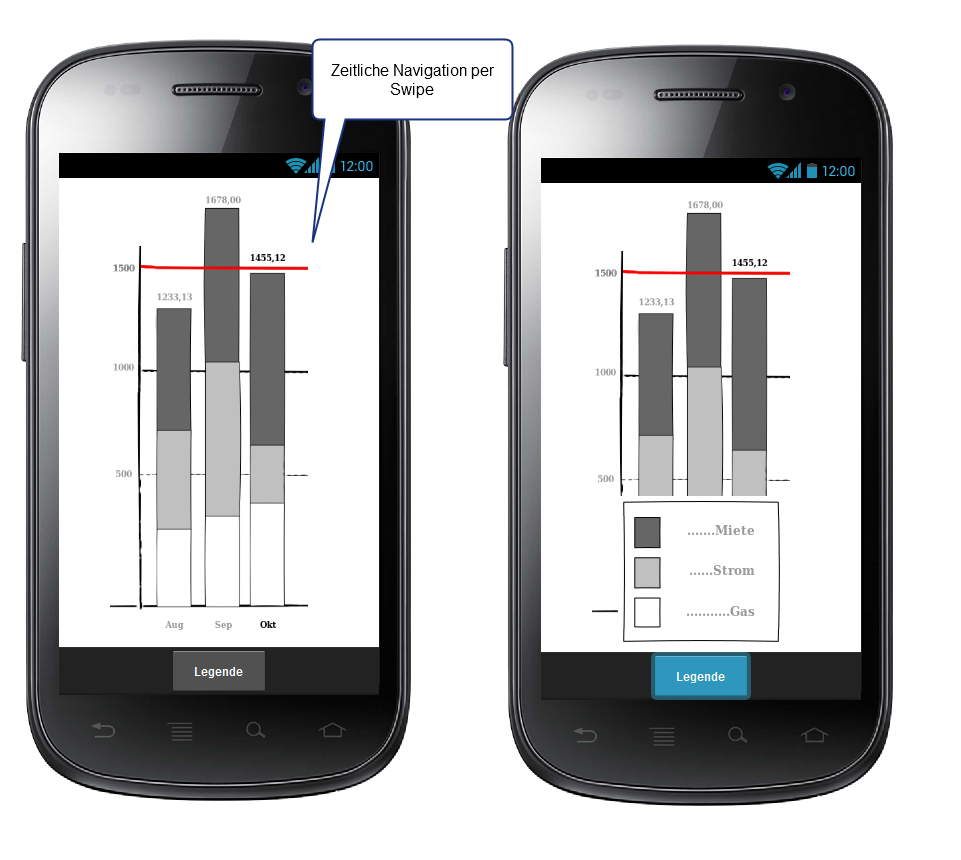
\includegraphics[width=8cm]{img/Statistik}
\caption{Statistik Screen}
\label{fig:statistik_screen}
\end{figure}

Hier ist ein S\"aulendiagramm zu sehen, das für 3 Monate jeweils eine S\"aule zeigt. Zur Unterscheidung der Kategorien sind diese farblich getrennt. Die zugeh\"orige Legende lässt sich schnell durch einen Button einblenden. Durch die „Swipe“-Geste nach links oder rechts kann der dargestellte Zeitraum navigiert werden.

\newpage
\subsection{Detailfragen}

\subsubsection{Frage 1}

\emph{Wie kann man Benutzer bei der Eingabe von Datensätzen unterstützen? Wie lassen sich Fehleingaben vermeiden? Wie werden diese Konzepte in Ihrem Prototypen realisiert?}

\vspace{2mm}

F\"ur den Benutzer muss immer klar erkennbar sein, welche Eingaben gerade
gefordert sind und wie diese erwartet werden. Ebenso muss man erkennen
k\"onnen wann eine Eingabe n\"otig ist.

Das l\"asst sich z.B. durch visuelle Affordances oder Constraints
erreichen. Wenn das User Interface erst keine falschen Eingaben zul\"asst,
k\"onnen auch keine gemacht werden.

Sowohl im Desktop als auch im Smartphone Interface sind Buttons, Textfelder
oder Drop-down-Men\"us hervorgehoben und falls notwendig beschriftet oder
mit einer Dummy-Eingabe, die das geforderte Format erkennen
l\"asst bef\"ullt (siehe Abbildung \ref{fig:eingabe_screen}). Zus\"atzlich
werden Eingabefelder, die gerade nicht sinnvoll sind ausgeblendet.

Bei der Eingabe eines Datums \"offnet sich automatisch ein Kalender, wo das
gew\"unschte Datum selektiert werden kann. Dadurch m\"ussen Horst und
Frauke nicht r\"atseln, welches Format ben\"otigt wird.

Zus\"atzlich werden Eingabefelder auf eine Breite beschr\"ankt, die
erkennen l\"asst was gefordert sein k\"onnte. So sind z.B. in der
Eingabezeile des Desktop-Interfaces die Spalten \glqq Betrag\grqq\space und
\glqq Datum\grqq\space schm\"aler als z.B. \glqq Beschreibung\grqq\space
(siehe Abbildung \ref{fig:web_details}).

Bei der Kategorie ist es m\"oglich eine neue zu erstellen oder eine alte zu
verwenden. Damit Horst, wenn er beispielsweise einen neuen Comic
eintr\"agt, nicht in die Verlegenheit kommt unabsichtlich
\glqq Comiv\grqq\space als Kategorie anzugeben, wird ihm \glqq Comic\grqq\space
bereits als m\"ogliche Eingabe angeboten.



\subsubsection{Frage 2}

\emph{Welche Informationen sind für Benutzer besonders wichtig und wie lässt sich
deren Bedeutung im System repräsentieren? Welche Such-/Filter-/Sortier-Funktio\-nen sind nützlich?}

\vspace{2mm}

Der Benutzer sollte auf einen Blick alle Ausgaben eines Monats sehen k\"onnen. Diese
werden auf der zentralen \"Ubersichtsseite chronologisch angeordnet dargestellt.

Ebenfalls sind einfache monatliche Zusammenfassungen wichtig; dazu wird in der
\"Ubersichtsseite am Ende jedes Monats eine Zusammenfassungszeile eingeblendet.
Die Zusammenfassung enth\"alt Informationen wie zum Beispiel die Summe aller monatlichen
Ausgaben, dessen Differenz zur festgelegten Budgetgrenze, und Vergleichswerte zu den Ausgaben
anderer Monate. Diese Zeile wird durch Schriftart und Hintergrundfarbe hervorgehoben.
Bei positiver Differenz (Grenze nicht \"uberschritten) ist die Differenz gr\"un dargestellt,
sonst rot.

Eintr\"age, die \"uber die Monatsgrenze hinausgehen werden durch rote Hintergrundfarbe
markiert.

Die Diagramme stellen vor allem Ausgaben pro Monat dar und sind als Balkendiagramme realisiert.
In diesem Zusammenhang ist nat\"urlich die Darstellung der monatlichen Obergrenze wichtig;
diese wird als Linie im Balkendiagramm eingezeichnet. Ebenfalls sind die Proportionen der Kategorien
von Interesse, deshalb wird ein Balken pro Kategorie eingef\"arbt.

Zur \"ubersichtlicheren Darstellung der Entwicklung von einzelnen Kategorien k\"onnen
diese auch in einem gefilterten Diagramm dargestellt werden (andere Kategorien werden
ausgeblendet).



\subsubsection{Frage 3}

\emph{Welche Möglichkeiten gibt es zur graphischen Aufbereitung der Daten 
(Grafiken, Kalender-Ansicht, etc.)? Wie werden diese Möglichkeiten in Ihrem Prototypen realisiert?}

\vspace{2mm}
Bei unseren Prototypen werden die Daten tabellarisch und in Form von Balkendiagrammen realisiert.
Das aktuelle Monat hat eine minimierte Darstellung mit den wichtigsten Kennzahlen in Form einer 
Tabelle (Abbildung \ref{fig:web_current_month}). Beim mobilen UI wird diese am Homescreen angezeigt
(Abbildung \ref{fig:smartphone_homescreen}).

\begin{figure}[htl]
\centering
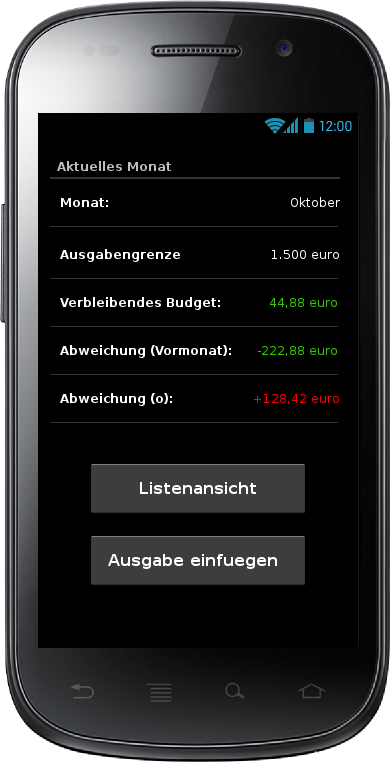
\includegraphics[width=4cm]{img/smartphone_homescreen}
\caption{Homescreen}
\label{fig:smartphone_homescreen}
\end{figure}

\newpage
\subsubsection{Frage 4}

\emph{Wie lässt sich eine sinnvolle Aufgabenteilung zwischen Desktop-UI und mobiler UI erreichen?
Welche Aufgaben haben bei der Verwendung zu Hause am Schreibtisch die höchste Priorität und welche
Aufgaben haben bei der Verwendung am Smartphone die höchste Priorität? Welche Formen der graphischen
Aufbereitung sind für den jeweiligen Anwendungskontext angemessen?}

\vspace{2mm}

Beim mobilen Userinterface wurde darauf geachtet, das nur die n\"otigsten Informationen und
Auswahlm\"oglichkeiten wie Buttons oder Eingabefelder am Bildschirm angezeitgt werden, da dieser,
im Gegensatz zum Desktopbildschirm, sehr klein ist. Es steht auch die schnelle und einfache
Eingabe einer get\"atigten Ausgabe im Vordergrund, diese hat also h\"ochste Priorit\"at.
Beim Desktop-UI wurde zwar auch auf \"Ubersichtlichkeit geachtet, man kann jedoch im Gegensatz
zum Bildschirm eines Smartphone's viel mehr Informationen darstellen und somit wird die h\"ochste
Priorit\"at auf das Verwalten, Auswerten und Eingeben von regelm\"assigen Ausgaben wie Miete, Strom,
Gas usw. gelegt. In Abbildung \ref{fig:smartphone_web_comparison} wird der Unterschied zwischen Desktop-UI-Eingabe und mobiler UI Eingabe gezeigt.

\begin{figure}[htl]
\centering
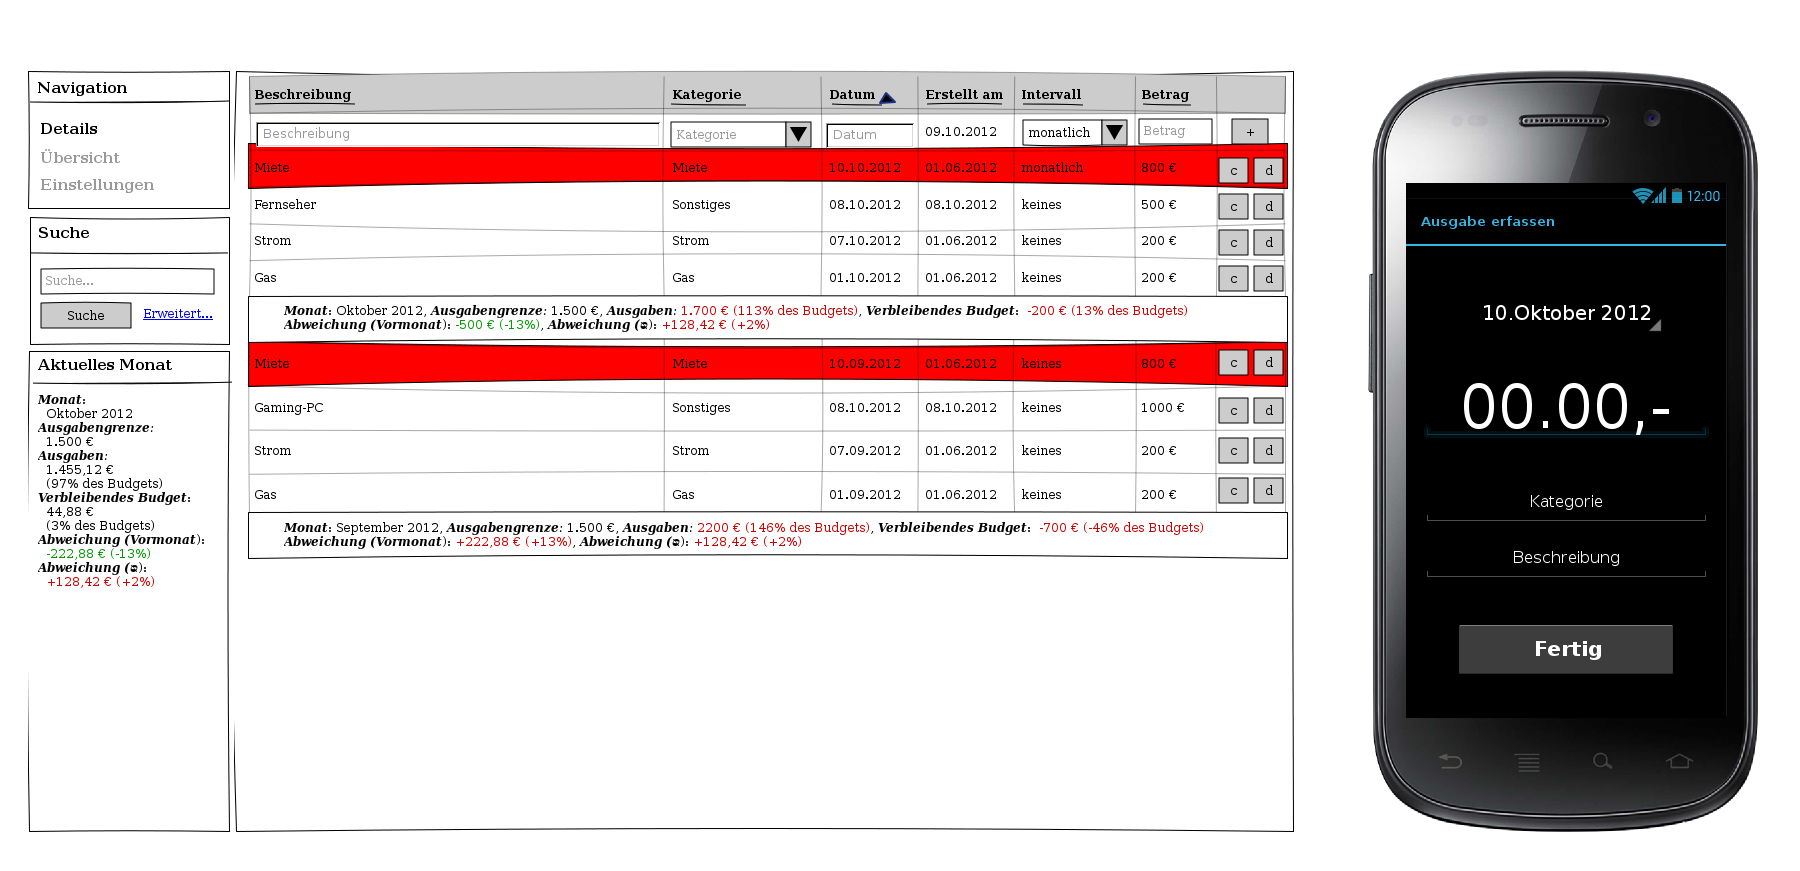
\includegraphics[width=\textwidth]{img/smartphone_web_comparison}
\caption{Eingabescreen Web/Smartphone}
\label{fig:smartphone_web_comparison}
\end{figure}
